% !TEX root = main.tex

\section{Anycast Deployment Strategies}\label{sec:anycast-services-utilization}
This section investigates the various deployment strategies used by anycast operators to deploy their services.
%
We use a single \laces snapshot, collected on February 18th, 2026, for this analysis.
On this day, \num{14346} IPv4 /24-prefixes and \num{13007} IPv6 /48-prefixes
were detected as anycast with confidence.
%

\subsection{Anycast Topology}\label{subsec:anycast-topology}
To evaluate the upstream ASes for anycast prefixes, we use data from \textit{bgp.tools} 
which contains \num{7442} routed prefixes (\num{4685} IPv4 and \num{2757} IPv6 prefixes) that cover the \laces{} /24-and /48-prefixes. 
%
We use \textit{bgp.tools} as they rely on many vantage points (3\,k+ BGP sessions~\cite{bgptools-features})
to maximize visibility for used upstreams.
Furthermore, unlike AS relationship data sets, the shared \dataset reports upstreams for each prefix separately.
%
For example, the University of Maryland (AS\,10886) has different upstreams for its anycast prefix 199.7.91.0/24 (D-root),
and its on-premise university ranges, where the AS relationship data would include upstreams for both prefixes.

For anycast prefixes,
we find tier-1 transit networks to be the most common upstreams (see Table~\ref{tab:anycast_upstreams} in Appendix~\ref{sec:anycast-upstreams}).
We also find
%\num{1745}
37\% of IPv4 and
%\num{806}
29\% of IPv6 routed prefixes with only a single upstream.
This is surprising, as one would expect anycast ASes to have
a large variety of upstreams due to their distributed nature.

\begin{figure}[t]
\centering
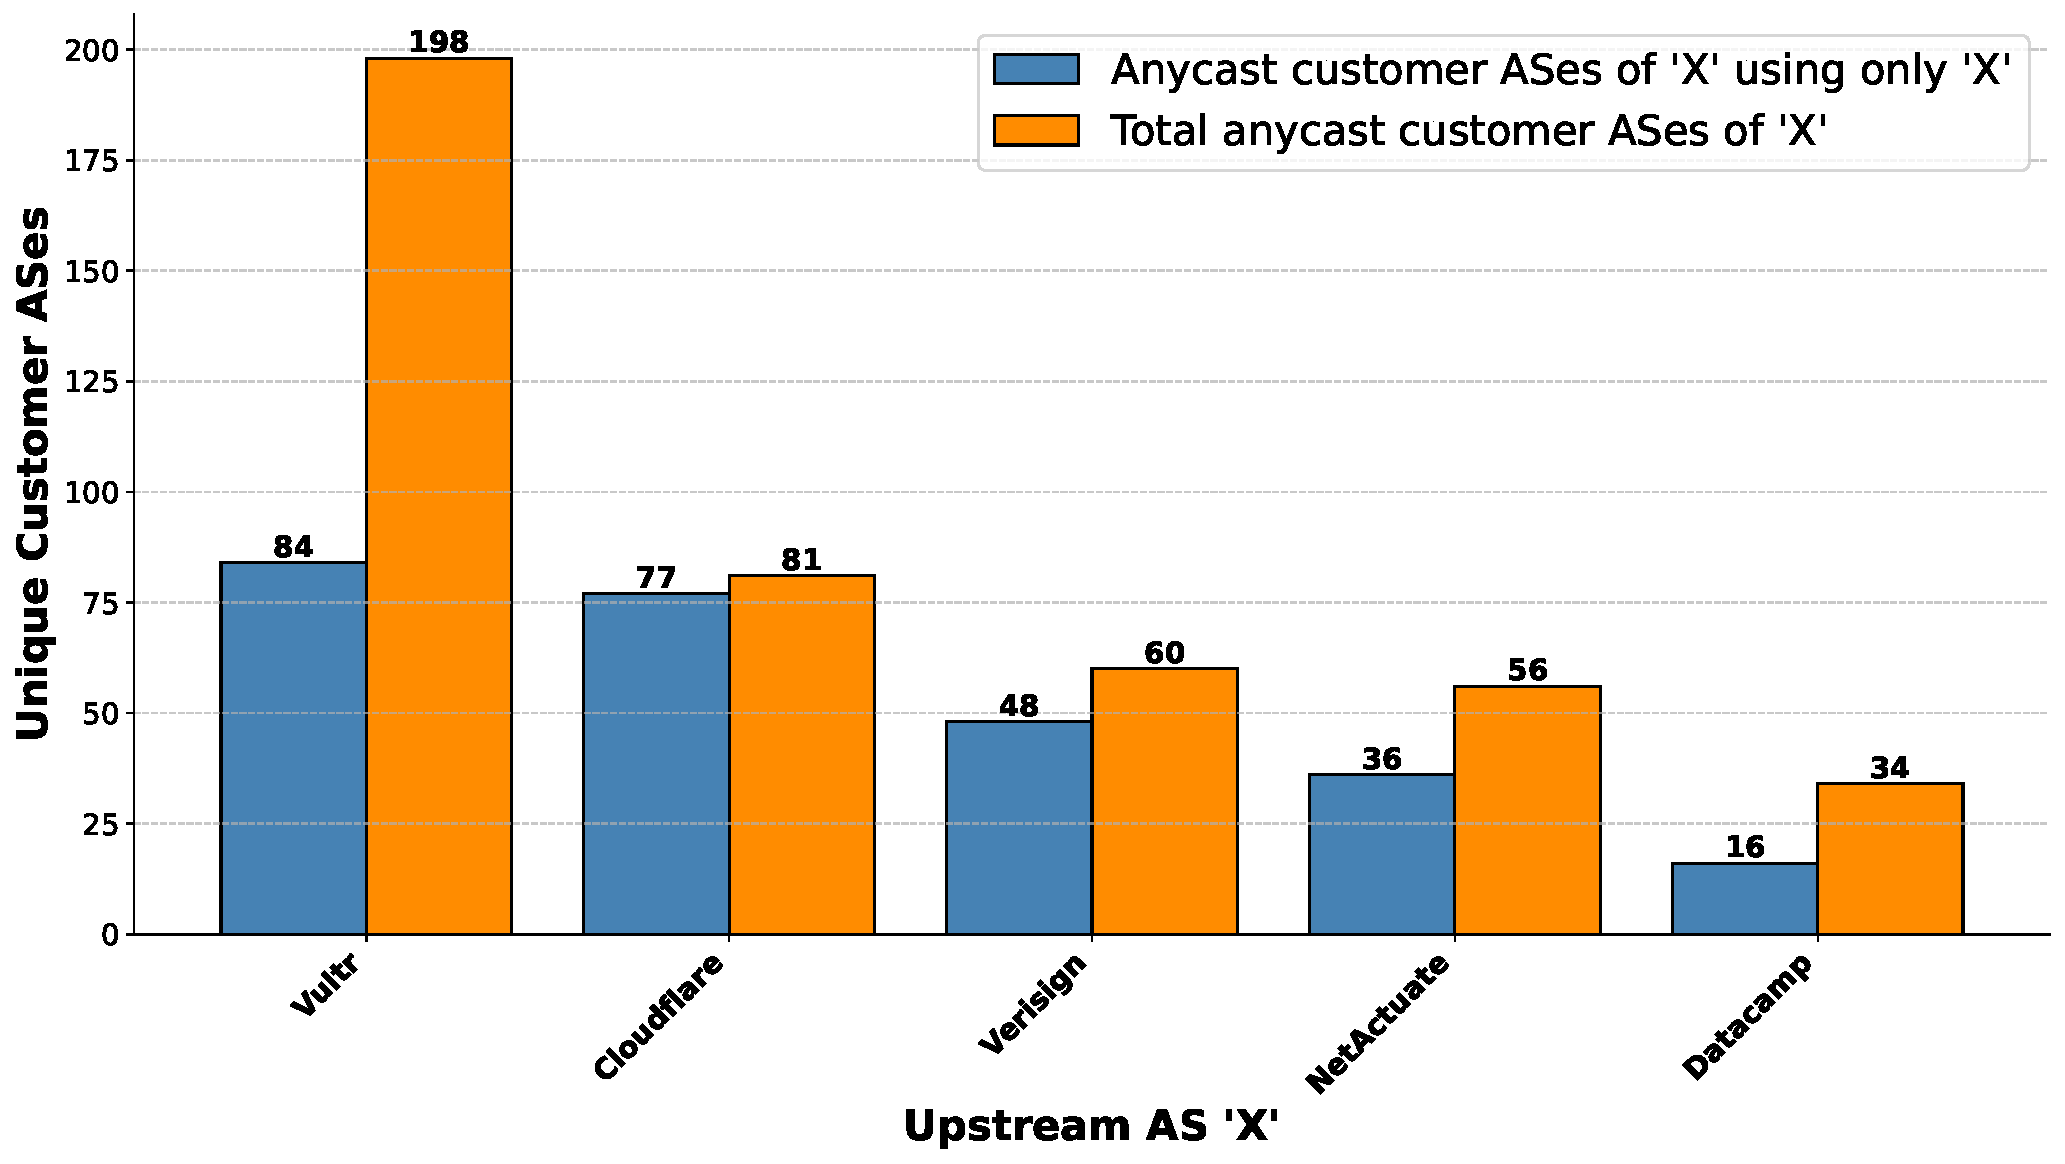
\includegraphics[width=\columnwidth]{./data/plots/byoip_customer_upstreams_ases}
\caption{
Most common upstreams for single-upstream anycast ASes.
}
\vspace*{-4mm}
\label{fig:single_upstream}
\end{figure}

~\cref{fig:single_upstream} plots the most frequent upstreams for single-upstream anycast ASes
alongside the total customer anycast ASes for that upstream.
%
These links mostly include customer-provider relationships for \gls{byoip} customers,
where operators announce their own ASN and prefix using a provider's infrastructure
(in which case the provider's ASN is the only upstream).

We find \num{198} ASes use Vultr as upstream to make use of anycast.
Furthermore, \num{84} out of these entirely use Vultr (as a single provider).  
%
Next, we have \num{77} ASes that replicate their services solely using Cloudflare and \num{36} that deploy entirely using NetActuate.
% NOTE: cloudflare and netactuate also provide ddos mitigation, and transit services (magic transit for example)

We also observe Verisign with \num{60} customer ASes,
which are
same-organization links for their Multi-Origin AS (MOAS) anycast infrastructure.
%
RFC~6382 describes using multiple ASNs for a single anycast prefix (one per \gls{pop})
via MOASes~\cite{rfc6382}.
%RFC~6382, describes the usage of a unique ASN for each anycast \gls{pop}~\cite{rfc6382}
%
This practice allows anycast operators,
\eg, to have a unique identifier for each PoP in routing data,
to assist with traffic engineering,
or to deploy an anycast service across multiple organizations.

Previous work by Sediqi et al.~\cite{moas-study} looked at long-lived MOASes, and found
they were rarely used for anycast.
%
We find similar results, as only \num{204} IPv4 and \num{111} IPv6 anycast prefixes have multiple AS origins.
%
Of these, 65\% consist of 2 origin ASes, 14\% have between 2 and 8 origins, and 35\% range from 8 to 15.
%
Lastly, we find that
most belong to Verisign (authoritative for many TLDs and author of RFC~6382).
%
%and DigiCert (a major certificate authority).
%Mimecast (an e-mail security company),
%Pearson (a large education company),
%and
%LeaseWeb (a large CDN).
We suspect the relatively low adoption of MOASes for anycast
is caused by the operational complexity of maintaining and deploying multiple ASes.

\subsection{Geographic Placement Strategies}\label{subsec:geographic-distribution}
Alongside detection, \laces also enumerates and geolocates anycast prefixes using iGreedy~\cite{igreedy}.
However, iGreedy's performance depends on the distribution of \glspl{vp} used
and has known limitations like struggling to differentiate between \glspl{pop} in close geographical proximity.
%
To mitigate these limitations, we only look whether an anycast AS has presence
within subregions (as defined by the United Nations~\cite{un_geoscheme})
that span large geographic areas where operator presence is more reliably detected in \laces.

\subsubsection{Global \gls{pop} placement}
\begin{figure}[t]
\centering
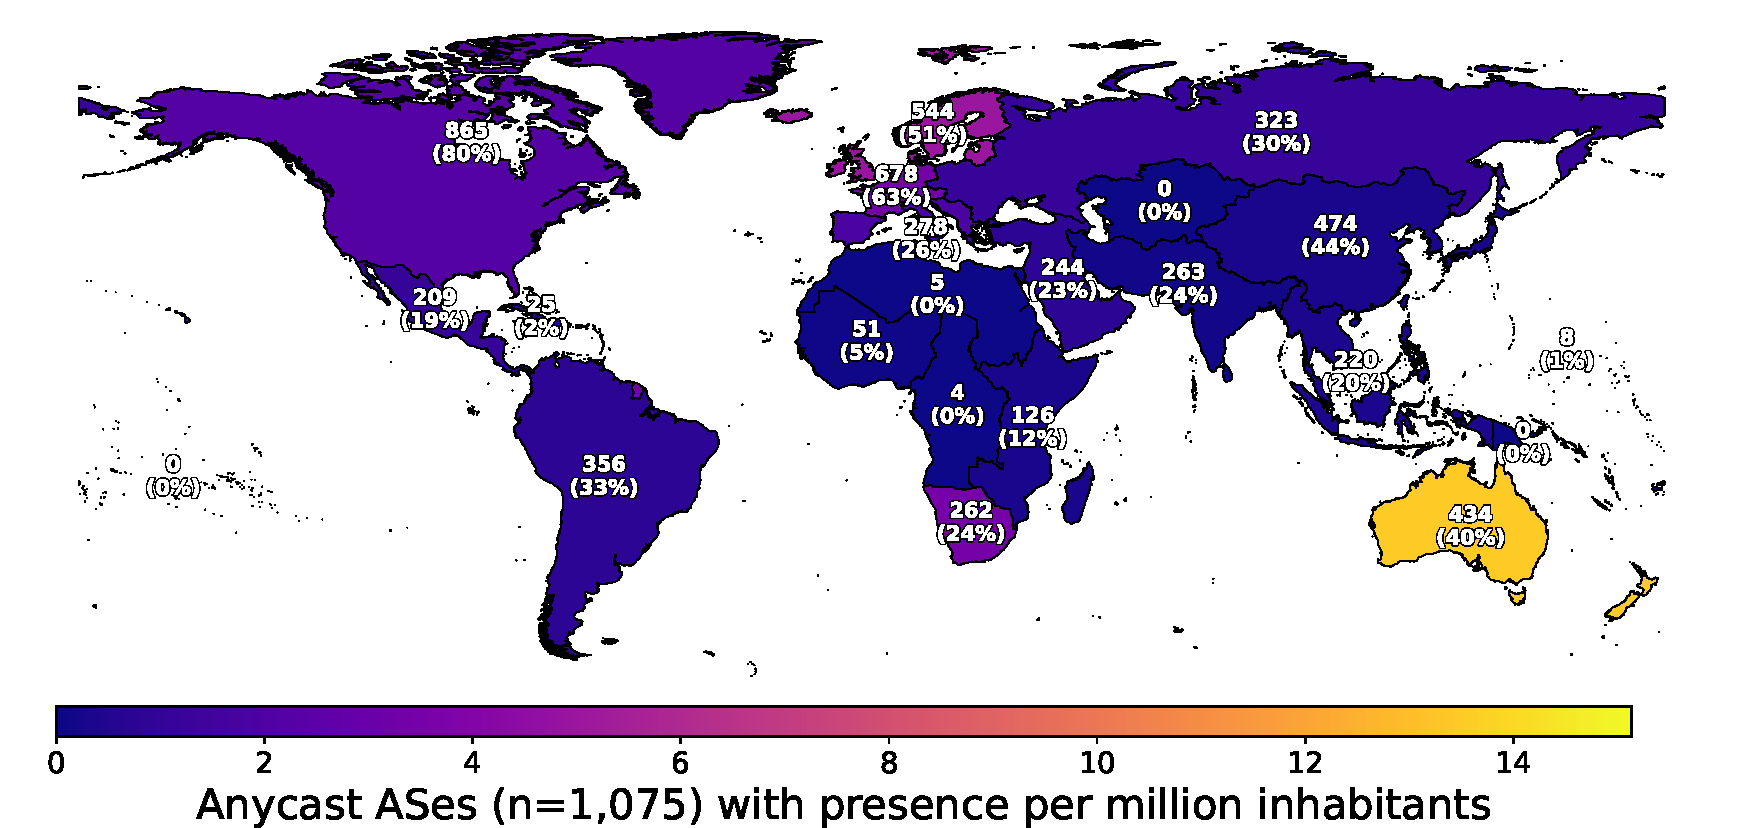
\includegraphics[width=\columnwidth]{./data/plots/map_subregion_heatmap_per_capita}
\caption{
    heatmap of the number of anycast ASes with presence in each subregion, normalized by millions of inhabitants.
}
\vspace*{-4mm}
\label{fig:a}
\end{figure}

~\cref{fig:a} shows the number of anycast ASes with presence in each subregion.
We find most operators have presence in North America (80\%), Western Europe (63\%), and Northern Europe (51\%).
%
Other subregions, such as Central America, Africa (except Southern Africa), Central Asia, and the Pacific Islands, have a sparse presence.
%

%
Next, looking at the normalized values based on the population count (using the population estimates of the UN~\cite{unwpp2024})
we find the Australia and New Zealand subregion to be the most represented by far.
%
We attribute this to the sparse population of this subregion, combined with its large digital economy.

South American ad Eastern Asia have a considerable number of ASes with presence
(33\% and 44\% respectively)
but are underserved when considering their large population.

These results show deployment differences where operators are likely to have presence in some subregions
but appear lacking in others.
%
We leave a more detailed analysis of anycast in underserved regions to future work

\subsubsection{Regional Anycast}

\begin{table}[tb]
    \centering
    \caption{Regional deployment scope of ASes (n=\num{1075}) with IPv4 anycast /24-prefixes (n=\num{14346}) observed by \laces.}
    \begin{tabular}{l r@{~}l r@{~}l}
        \toprule
        Deployment Scope & \multicolumn{2}{c}{ASes} & \multicolumn{2}{c}{/24-Prefixes} \\
        \midrule
        Global (multi-continent)            & \num{794} & (74\%) & \num{13135} & (92\%) \\
        Single continent                    & \num{381} & (35\%) & \num{1211} & (8\%) \\
        \quad Single country                & \num{245} & (23\%) & \num{769} & (5\%) \\
        \midrule
        \multicolumn{5}{l}{\textit{Single-continent deployments by region (ASes=\num{381}, /24s=\num{1211})}} \\
        \midrule
        \quad North America                 & \num{196} & (51\%) & \num{724} & (60\%) \\
        \quad Europe                        & \num{119} & (31\%) & \num{223} & (18\%) \\
        \quad Asia                          & \num{51} & (13\%) & \num{128} & (11\%) \\
        \quad Oceania                       & \num{46} & (12\%) & \num{122} & (10\%) \\
        \quad South America                 & \num{10} & (3\%) & \num{12} & (1\%) \\
        \quad Africa                        & \num{2} & (1\%) & \num{2} & (0\%) \\
%        \midrule
%        \multicolumn{5}{l}{\textit{Single-country deployments by country (ASes=\num{245}, /24s=\num{769})}} \\
%        \midrule
%        \quad United States                 & \num{166} & (68\%) & \num{570} & (74\%) \\
%        \quad Australia                     & \num{36} & (15\%) & \num{104} & (14\%) \\
%        \quad France                        & \num{11} & (4\%) & \num{19} & (2\%) \\
%        \quad Canada                        & \num{7} & (3\%) & \num{9} & (1\%) \\
%        \quad Japan                         & \num{7} & (3\%) & \num{16} & (2\%) \\
%        \quad United Kingdom                & \num{6} & (2\%) & \num{14} & (2\%) \\
%        \quad India                         & \num{5} & (2\%) & \num{5} & (1\%) \\
%        \quad Russia                        & \num{5} & (2\%) & \num{6} & (1\%) \\
%        \quad New Zealand                   & \num{4} & (2\%) & \num{11} & (1\%) \\
%        \quad Brazil                        & \num{3} & (1\%) & \num{8} & (1\%) \\
%        \quad Spain                         & \num{3} & (1\%) & \num{5} & (1\%) \\
%        \quad Switzerland                   & \num{1} & (0\%) & \num{2} & (0\%) \\
        \bottomrule
    \end{tabular}
    \label{tab:anycast_regional}
    \vspace*{-4mm}
\end{table}

\laces covers \num{1075} ASes deploying IPv4 anycast,
some of which are ``regional'', which we define as anycasted within a single continent or country.
~\cref{tab:anycast_regional} provides a breakdown of the geographic deployment scope of anycast ASes and prefixes.

We find 74\% of ASes have at least one prefix with global presence (\ie, spanning multiple continents),
and 35\% have a prefix within a continent.
%
For these ASes announcing prefixes within a single continent,
we find 51\% have prefixes confined to North America,
31\% confined to Europe,
13\% confined to Asia,
12\% confined to Oceania,
and less than 5\% confined to South America and Africa.
%
This shows many ASes deploy regional anycast
and highlights the bias of operators to deploy in North America and Europe
whereas few deploy inside of South America and Africa.


%
Interestingly, \num{23} ASes (mostly CDNs) announce regional anycast prefixes within multiple continents (see ~\cref{tab:anycast_multi_continent} in Appendix~\ref{sec:regional-anycast}).
For example, AWS (AS\,16509) has distinct regional deployments in five continents.

\subsection{IP utilization}\label{subsec:hypergiant-dominance}

Unlike previous work,
that only measured a single IP address per prefix~\cite{CicaleseEtAl_CharacterizingIPv4Anycast_2015},
we scan prefixes in their entirety
allowing us to assess the IP utilization of anycast.
In total, our scanning reveals
\num{1.77e6}
addresses with active services within \laces prefixes.
%
These prefixes cover \num{1223} distinct ASes of which
\num{1075} announce IPv4, \num{579} announce IPv6 anycast,
and \num{431} announce both IPv4 and IPv6 anycast.
%
However, as stated by Hendriks et al.~\laces has limited coverage for IPv6 due to hitlist limitations~\cite{Hendriks_LACeS_An_Open_2025},
and we suspect the actual number of ASes announcing IPv6 anycast to be higher.

% OLD TABLE (OCT 2024)
%\begin{table}
%\caption{Top 10 anycast ASNs by number of /24s}
%\begin{tabular}{rlrrrr}
%\toprule
%ASN & Name & Active IPs & /24-prefixes & BGP-prefixes & IP utilization \\
%\midrule
%396982 & Google Cloud & 826,588 & 3,351 & 146 & 96.36\% \\ % TODO expanded by 20% ish
%13335 & Cloudflare & 746,556 & 3,088 & 348 & 94.44\% \\ largely the same
%16509 & Amazon & 112,578 & 1,042 & 227 & 42.20\% \\ stayed the same
%54113 & Fastly & 115,122 & 454 & 50 & 99.05\% \\ % TODO doubled in number of /24s
%209242 & Cloudflare & 66,527 & 272 & 226 & 95.54\% \\ stayed the same
%12041 & Afilias & 2,075 & 224 & 224 & 3.62\% \\ stayed the same
%40509 & Fly.io & 19,949 & 220 & 115 & 35.42\% \\ stayed the same
%15169 & Google & 50,877 & 219 & 19 & 90.75\% \\ -> TODO what happened?
%15967 & NetArt Group & 46,904 & 191 & 41 & 95.93\% \\
%15133 & EdgeCast & 22,785 & 151 & 151 & 58.94\% \\ -> TODO what happened to EdgeCast? They reduced their deployment?
%\bottomrule
%\end{tabular}\label{tab:top_ases}
%\end{table}
%\begin{table}
%\label{tab:top_ases}
%\begin{tabular}{rlrrr}
%\toprule
%ASN & Organization & /24-prefixes & Active IPs & IP Utilization \\
%\midrule
%396982 & Google & 4,115 & 1,001,503 & 95.07\% \\
%13335 & Cloudflare & 2,712 & 653,999 & 94.20\% \\
%16509 & Amazon & 1,140 & 116,489 & 39.92\% \\
%54113 & Fastly & 837 & 212,937 & 99.38\% \\
%209242 & Cloudflare & 281 & 67,188 & 93.40\% \\
%12041 & Afilias & 223 & 2,116 & 3.71\% \\
%40509 & Fly.io & 219 & 20,000 & 35.67\% \\
%15967 & NetArtGroup & 195 & 47,945 & 96.04\% \\
%63911 & NetActuate & 105 & 1,151 & 4.28\% \\
%16276 & OVH & 99 & 12,415 & 48.99\% \\
%\bottomrule
%\end{tabular}
%    \caption{Number of active IPs and IP Utilization for the ten largest anycast ASNs by number of /24s.}
%\end{table}

% OLD RESULTS 4 FEB
%\begin{table}[tb]
%    \begin{tabular}{lrrrr}
%        \toprule
%        Org (ASN) & /24s & Active IPs & Active IP ratio & HRP ratio \\
%        \midrule
%        Cloudflare (13335) & 2,866 & 657,587 & 0.896 & 0.989 \\
%        Google (396982) & 4,319 & 262,845 & 0.238 & 0.974 \\
%        Fastly (54113) & 830 & 210,443 & 0.990 & 0.990 \\
%        AWS (16509) & 1,589 & 130,649 & 0.321 & 0.245 \\
%        Cloudflare (209242) & 268 & 59,822 & 0.872 & 0.978 \\
%        Fly.io (40509) & 223 & 21,711 & 0.380 & 1.000 \\
%        GoDaddy (398787) & 64 & 16,383 & 1.000 & 1.000 \\
%        AceVille (139341) & 115 & 12,943 & 0.440 & 0.835 \\
%        Nazwa.pl (15967) & 195 & 11,741 & 0.235 & 0.959 \\
%        Afilias (207266) & 82 & 11,142 & 0.531 & 0.061 \\
%        \bottomrule
%    \end{tabular}
%    \caption{Largest ASes by number of active IPs,
%        alongside the number of /24s
%        and Active IP \& HRP ratios.
%    }
%    \label{tab:top_ases}
%\end{table}

% RESULTS 18 FEB
\begin{table}[tb]
    \centering
    \caption{Largest ASes by number of active IPs,
        alongside the number of /24s
        and active IP \& HRP ratios.
    }
    \begin{tabular}{lrrrr}
        \toprule
        Org (ASN) & Active IPs & /24s & \makecell{Active \\ IP ratio} & HRP Ratio \\
        \midrule
        Cloudflare (13335) & \num{658e3} & \num{2866} & 0.896 & 0.989 \\
        Google (396982) & \num{492e3} & \num{4298} & 0.447 & 0.973 \\
        Fastly (54113) & \num{209e3} & \num{827} & 0.989 & 0.990 \\
        AWS (16509) & \num{133e3} & \num{1603} & 0.325 & 0.260 \\
        Cloudflare (209242) & \num{60e3} & \num{270} & 0.862 & 0.967 \\
        Fly.io (40509) & \num{22e3} & \num{223} & 0.387 & 1.000 \\
        GoDaddy (398787) & \num{16e3} & \num{64} & 1.000 & 1.000 \\
        AceVille (139341) & \num{13e3} & \num{118} & 0.430 & 0.805 \\
        Vercara (12008) & \num{12e3} & \num{98} & 0.459 & 0.449 \\
        Nazwa.pl (15967) & \num{11e3} & \num{195} & 0.224 & 0.959 \\
        \bottomrule
    \end{tabular}
    \label{tab:top_ases}
    \vspace*{-4mm}
\end{table}

Table~\ref{tab:top_ases} shows the largest ASes by number of anycasted IPv4 addresses with active services found using our pipeline
alongside the number of /24-prefixes they originate.

We also include the IP utilization and HRP ratios.
The former is the ratio of active IPs, \ie with detected active services,
the latter is the ratio of HRP /24-prefixes~\cite{SattlerEtAl_PackedBrimInvestigating_2023}.
%
In total, \num{9.7e3} /24s (68\%) are classified as HRP
for which we find an average IP utilization of 42\%
compared to 12\% for non-HRP prefixes.
Thus, while for HRPs a majority of IP addresses result in a successful TCP handshake,
a valid service can only be identified for 42\% of addresses.

Hendriks \etal~showed a clear dominance of so-called hypergiants
where the top 5 ASes announce roughly two-thirds of all anycast /24-prefixes~\cite{Hendriks_LACeS_An_Open_2025}.
We find this is even more centralized as 88\% of active IPs are originated by these top 5 ASes,
due to their high IP utilization.

For Cloudflare, Fastly, and GoDaddy, we find high IP utilization and HRP ratios,
with Cloudflare originating 37\% of active anycast IP addresses.
%
Despite an IP utilization of 45\%, Google has the second-most active IP addresses (28\%) as they originate the most /24-prefixes.
%
This suggests Google can provision the same number of services using fewer prefixes.

For IPv6, we find Cloudflare (AS\,209242) to originate 49\% of /48s (see Table~\ref{tab:top_ases_v6} in Appendix~\ref{sec:ipv6-anycast}.
We do not know the active IP ratio for IPv6 prefixes, due to the large number of addresses in /48-prefixes, which makes scanning impossible.

These results show that most active anycast IPs are hosted by a few ASes that originate the majority of prefixes,
which are also classified as HRP with high IP utilization.
%
For this reason, we will separately consider HRP prefixes in parts of our presented results.

\begin{figure}[t]
\centering
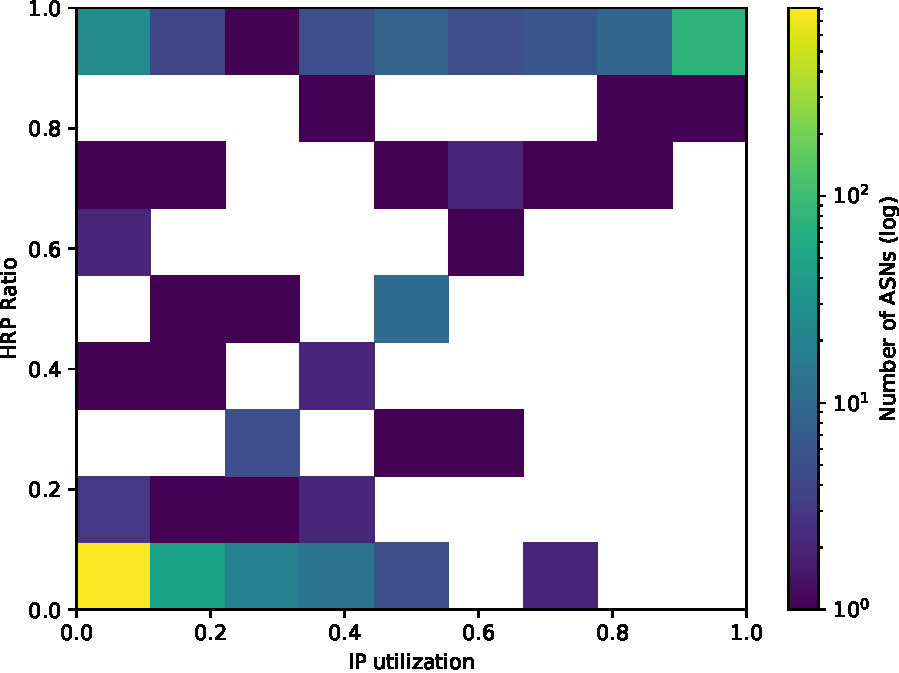
\includegraphics[width=\columnwidth]{./data/plots/as_ip_hrp_heatmap}
\caption{
    Heatmap of HRP ratio against active IP ratio for anycast ASes (IPv4 only).
}
\vspace*{-4mm}
\label{fig:heatmap}
\end{figure}

~\cref{fig:heatmap} shows the correlation between HRP and active IP ratios for IPv4 anycast ASes.
We find the majority of ASes have a low active IP and HRP ratio (bottom left),
as we discuss later in \S\ref{sec:results}, these are mostly ASes deploying DNS\@.
%
Next, we find a considerable number of ASes with high HRP and active IP ratio (top right),
these are hypergiant ASes like Cloudflare, Fastly, and GoDaddy, as seen in Table~\ref{tab:top_ases}.
%

Interestingly, we observe \num{31} ASes that deploy HRP with few active IPs (top left), mostly CDN operators based on manual inspection.
%
In the bottom-right corner, we find FastHosts (AS\,15418) and InternetNamesForBusiness (AS\,14116), both with high IP utilization and no HRP.
They use anycast DNS infrastructure as domain registrars (not classified as HRP, which is based on open TCP ports).
%
In the center, we find \num{13} ASes that deploy a near-even split of HRP and non-HRP prefixes.
The largest of which are Vercara (AS\,12008), a subsidiary of DigiCert,
and Alibaba (AS\,24429), both offering a large variety of service,s including anycasted DNS and DDoS protection.
% https://www.alibabacloud.com/help/en/anycast-eip/user-guide/getting-started -> not replicated (tunneling to single datacenter)
